% =====================================================================
%  CAPÍTULO 7 — RESULTADOS, VALIDAÇÃO E DISCUSSÃO
% =====================================================================

\chapter{RESULTADOS, VALIDAÇÃO E DISCUSSÃO}
\label{cap:resultados}

Este capítulo apresenta o que foi observado durante o desenvolvimento e a
avaliação do \argus{}. O objetivo não é demonstrar superioridade sobre
plataformas comerciais, mas verificar se o artefato sustenta o fluxo proposto,
quais requisitos foram atendidos e quais permanecem em aberto. A apresentação
distingue evidência de construção, evidência de demonstração e evidência de
avaliação, conforme definido no Capítulo~\ref{cap:metodologia}.

\section{Estratégia de avaliação}
\label{sec:estrategia-avaliacao}

A avaliação foi organizada em quatro frentes complementares:

\begin{itemize}
    \item \textbf{funcional}: no desktop, execução do fluxo completo (GPX,
        sensores, rolo, sessão, análise e exportação); no Android, execução
        da sessão ao vivo; conferência contra os requisitos da
        Tabela~\ref{tab:requisitos};
    \item \textbf{plataformas}: verificação de compilação e uso em
        \textit{desktop} Windows/Linux e em telefone Android, com profundidade
        funcional diferente e registro explícito do que não foi validado;
    \item \textbf{dados}: inspeção do acervo de arquivos \texttt{.FIT} e
        verificação de aceitação por Strava e Intervals.icu em testes de
        exportação;
    \item \textbf{piloto}: uso do sistema pelo próprio autor em sessões com
        rolo e sensor de frequência cardíaca reais, com diário de observações.
\end{itemize}

A avaliação não inclui medição instrumentada de latência, consumo de memória ou
estabilidade por longa duração. Essas grandezas são relevantes, mas exigiriam
instrumentação e protocolo próprios; por isso, não são apresentadas como
resultados. A ausência é declarada e retomada nas limitações.

\section{Avaliação funcional}
\label{sec:avaliacao-funcional}

As funcionalidades foram exercitadas manualmente ao longo do desenvolvimento,
em sessões livres, treinos estruturados e modos de evento. A
Tabela~\ref{tab:avaliacao-funcional} relaciona os requisitos aos tipos de
evidência observados e ao status atribuído.

\begin{table}[htbp]
    \centering
    \caption{Síntese da avaliação funcional}
    \label{tab:avaliacao-funcional}
    \footnotesize
    \renewcommand{\arraystretch}{1.15}
    \setlength{\tabcolsep}{4pt}
    \begin{tabular}{@{}>{\raggedright\arraybackslash}p{1.3cm}
        >{\raggedright\arraybackslash}p{5.3cm}
        >{\raggedright\arraybackslash}p{5.4cm}
        >{\raggedright\arraybackslash}p{2.8cm}@{}}
        \toprule
        \textbf{ID} & \textbf{Evidência observada} &
        \textbf{Resultado} & \textbf{Status} \\
        \midrule
        RF01 & GPX importado, perfil e distância conferidos em rotas do
        acervo & Perfil e mapa coerentes com o arquivo & Verificado \\
        RF02 & Sessões com rolo em modo simulação e ERG & Resistência
        alterou com a inclinação nos equipamentos testados & Verificado \\
        RF03 & Sessões com sensor de FC, potência e cadência & No desktop, telemetria
        exibida e gravada por notificação BLE; no Android, HUD ao vivo &
        Verificado \\
        RF04 & Cálculo de NP, IF, TSS, TRIMP, PMC, HRR e desacoplamento &
        No desktop, métricas disponíveis e fórmulas documentadas &
        Implementado, sem validação clínica \\
        RF05 & Reinício do aplicativo e troca de perfil & No desktop, dados
        preservados e perfis isolados no SQLite & Verificado \\
        RF06 & Exportação FIT e envio ao Strava/Intervals.icu & No desktop,
        arquivos aceitos nos testes realizados & Verificado em amostra \\
        RF07 & Execução em Windows, Linux e Android & Fluxo completo no
        desktop; sessão ao vivo no Android, com adaptações de layout &
        Verificado \\
        RF08 & Caso Geraardsbergen--Leberg & No desktop, importação, perfil,
        sessão e análise do FIT; no Android, perfil e sessão ao vivo &
        Demonstrado \\
        \bottomrule
    \end{tabular}
    \vspace{0.2cm}
    \par\small Fonte: autoria própria.
\end{table}

As Figuras~\ref{fig:screenshot-career} e~\ref{fig:screenshot-history} mostram
duas telas usadas na conferência: o painel de carga com PMC e o histórico de
atividades com as métricas calculadas. Elas são evidências de interface, não
provas de exatidão fisiológica.

\begin{figure}[htbp]
    \centering
    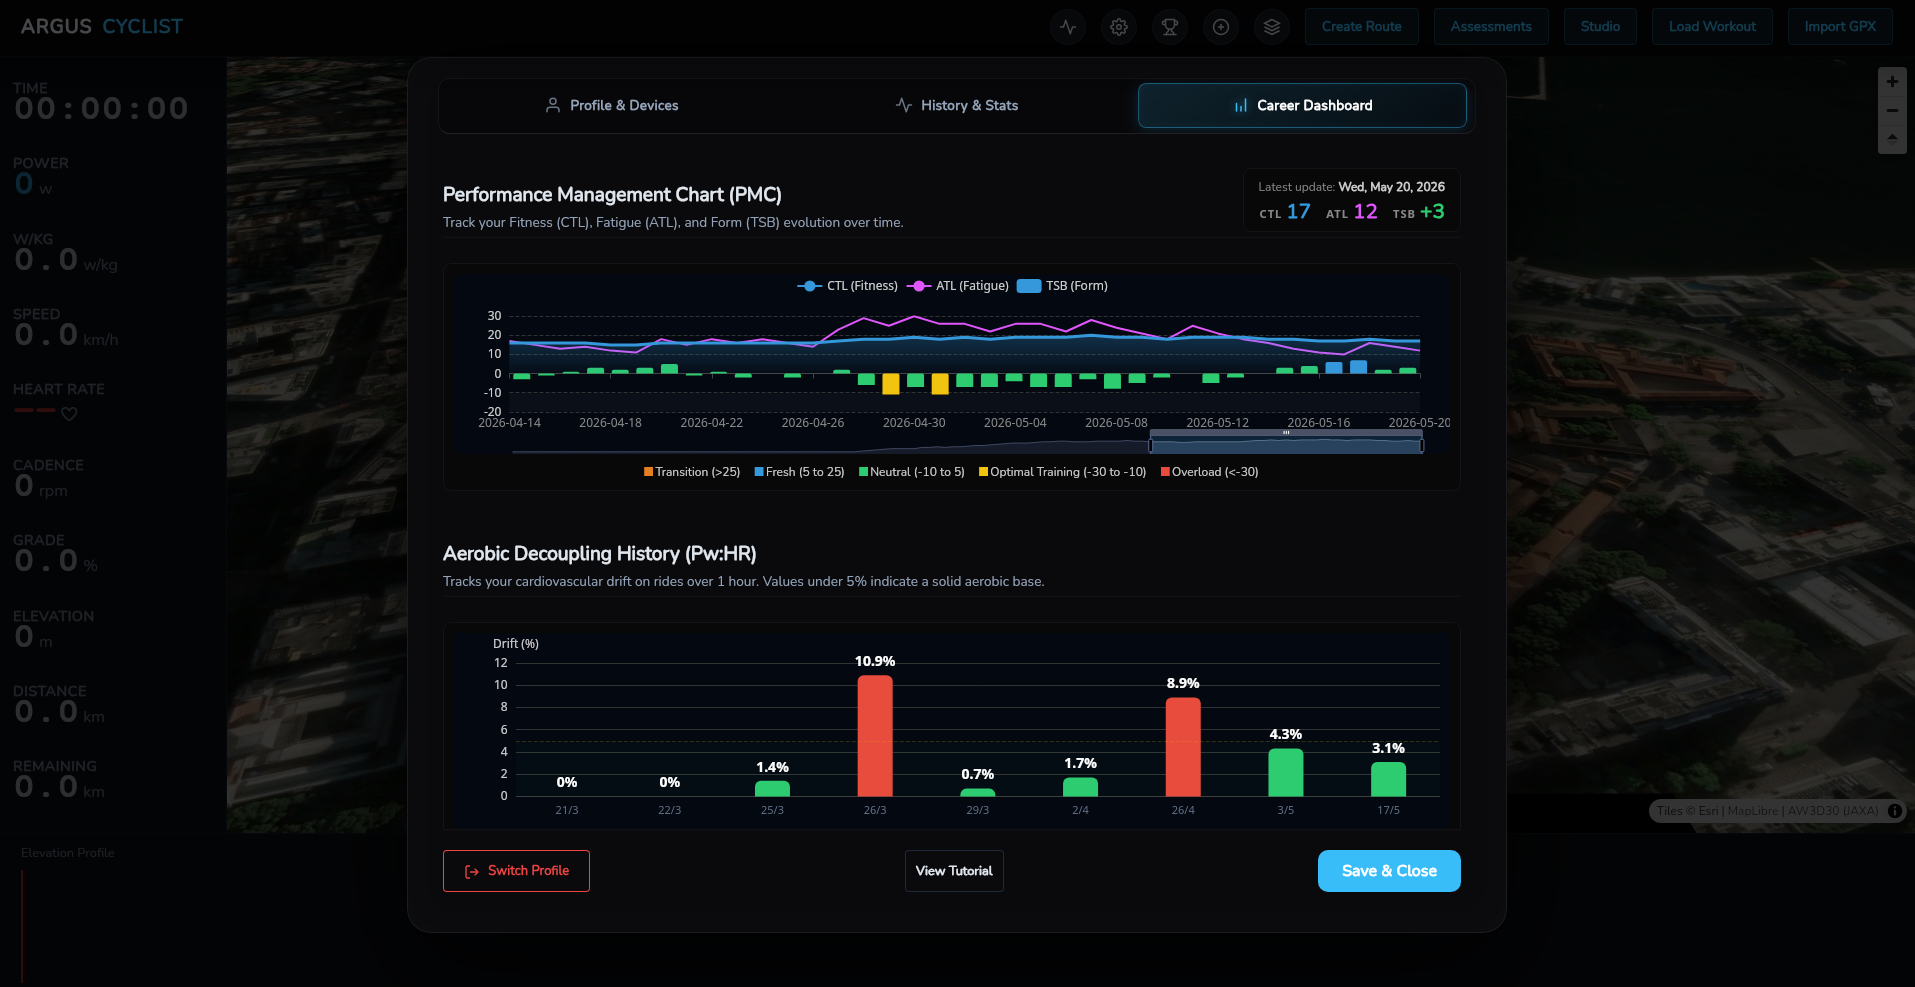
\includegraphics[width=0.85\textwidth]{figuras/screenshot-04-career}
    \caption{\textit{Dashboard} de carreira: PMC (CTL/ATL/TSB) e desvio cardiovascular}
    \label{fig:screenshot-career}
    \small Fonte: autoria própria.
\end{figure}

\begin{figure}[htbp]
    \centering
    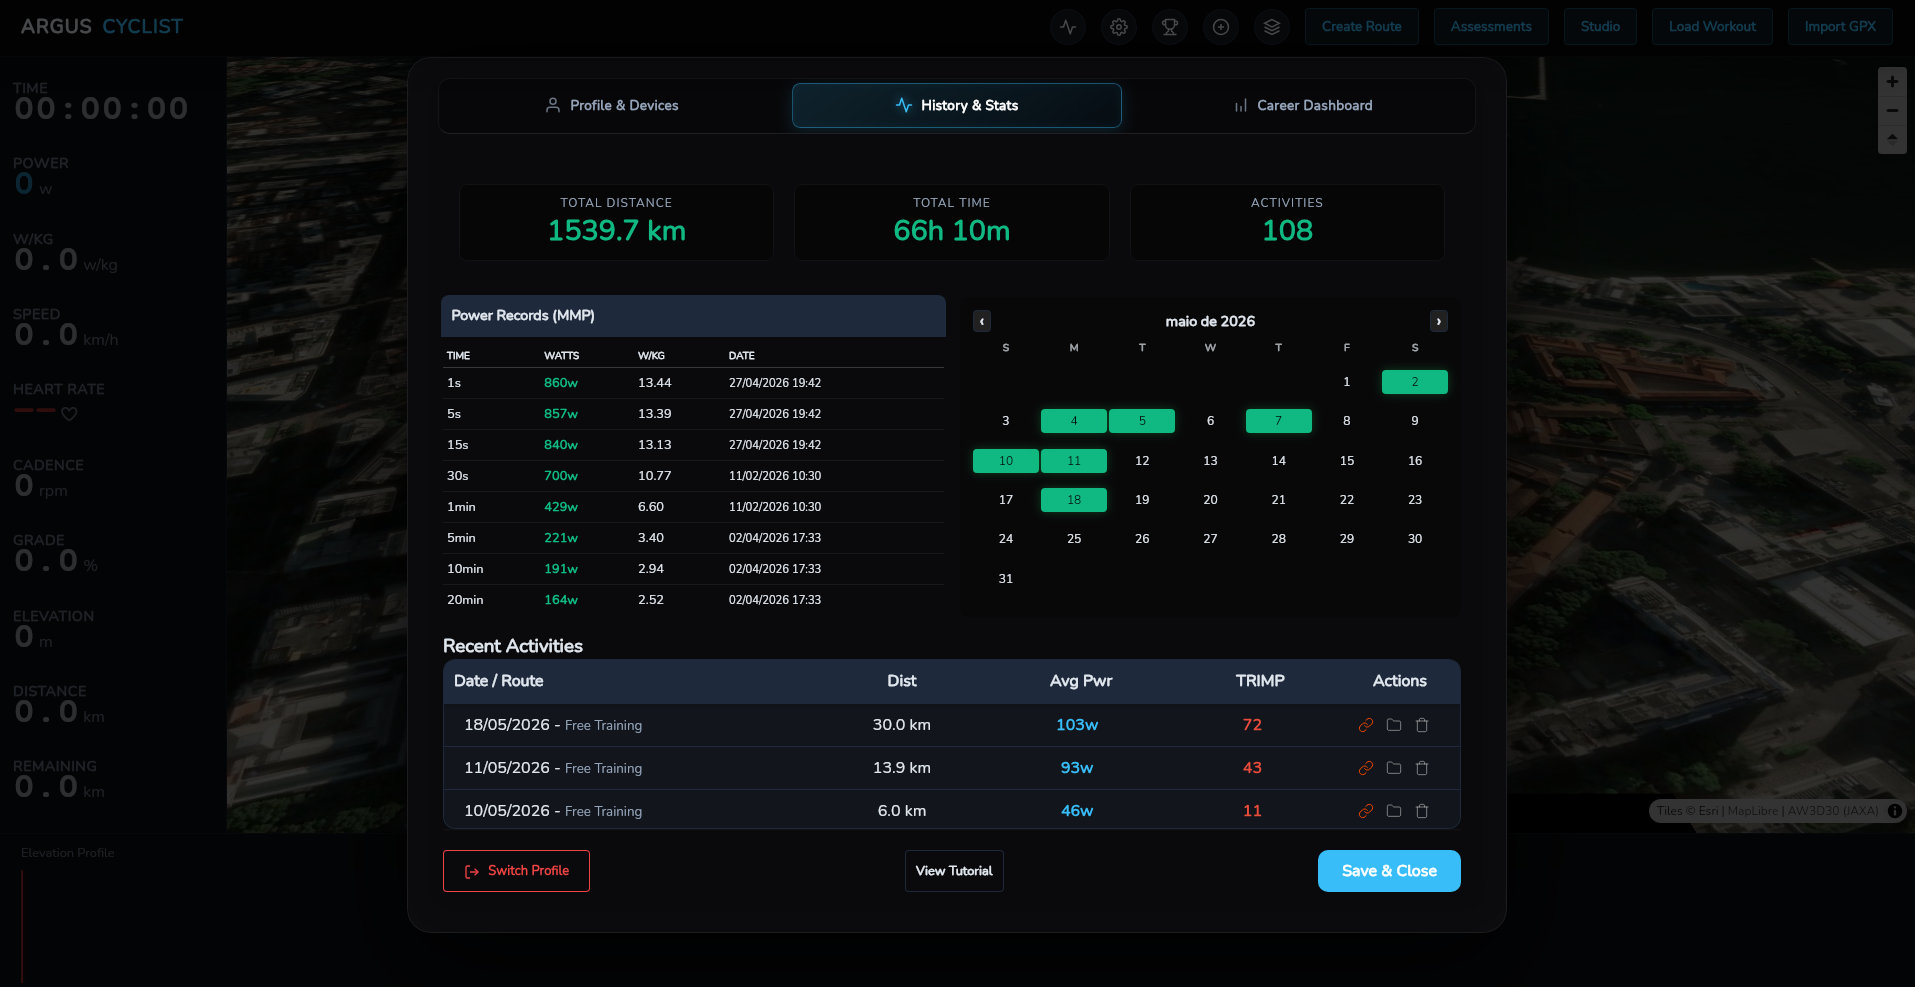
\includegraphics[width=0.85\textwidth]{figuras/screenshot-03-history}
    \caption{Histórico de atividades com métricas fisiológicas}
    \label{fig:screenshot-history}
    \small Fonte: autoria própria.
\end{figure}

\section{Avaliação de plataformas}
\label{sec:avaliacao-plataformas}

A Tabela~\ref{tab:plataformas} separa o que foi efetivamente exercitado do que
existe apenas como preparação. Essa distinção é importante porque o título do
trabalho usa a palavra ``multiplataforma'': ela se sustenta nas plataformas
validadas, não em uma promessa de cobertura universal.

\begin{table}[htbp]
    \centering
    \caption{Status de validação por plataforma}
    \label{tab:plataformas}
    \footnotesize
    \renewcommand{\arraystretch}{1.15}
    \setlength{\tabcolsep}{4pt}
    \begin{tabular}{@{}>{\raggedright\arraybackslash}p{2.8cm}
        >{\raggedright\arraybackslash}p{3.4cm}
        >{\raggedright\arraybackslash}p{6.2cm}
        >{\raggedright\arraybackslash}p{2.6cm}@{}}
        \toprule
        \textbf{Plataforma} & \textbf{Ambiente testado} &
        \textbf{O que foi verificado} & \textbf{Status} \\
        \midrule
        Windows & Windows 11, desktop & Compilação Wails, BLE, rolo,
        sessão, FIT e integrações & Validado \\
        Linux & Arch Linux, notebook & Compilação Wails, BLE, sessão e FIT &
        Validado \\
        Android & Telefone Android, Capacitor & Compilação, BLE nativo, layout
        responsivo e sessão ao vivo & Validado como modo ao vivo \\
        macOS & Não testado & Compilação prevista pelo Wails &
        Não validado \\
        iOS/iPadOS & Não compilado & Estrutura Capacitor preparada &
        Não validado \\
        Tablet Android & Não testado & Layout responsivo projetado &
        Não validado \\
        \bottomrule
    \end{tabular}
    \vspace{0.2cm}
    \par\small Fonte: autoria própria.
\end{table}

A validação em Android foi feita em telefone, não em tablet. O layout usa
\textit{breakpoints} e reorganização de painéis, mas isso não equivale a um
teste de usabilidade em tela grande. Da mesma forma, a existência de código
iOS no projeto Capacitor não significa que o aplicativo tenha sido compilado,
assinado ou executado em um dispositivo Apple.

\section{Integridade dos dados exportados}
\label{sec:avaliacao-dados}

O diretório de trabalho reúne 274 arquivos \texttt{.FIT}, 23 arquivos GPX e 5
arquivos ZWO, acumulados durante o desenvolvimento e as sessões de teste. Esse
acervo documenta a variedade de percursos e de sessões, mas não é uma amostra
aleatória nem um conjunto controlado.

Nos testes de exportação, arquivos gerados pelo \argus{} foram aceitos pelo
Strava e pelo Intervals.icu. A conferência manual comparou distância, duração,
potência média, elevação e frequência cardíaca entre o aplicativo e as
plataformas de destino. A aceitação por Strava e Intervals.icu é a evidência de
interoperabilidade disponível; a validação formal com o validador oficial do FIT
SDK permanece como trabalho futuro. A comparação estatística com um sistema de
referência independente também permanece como trabalho futuro. A
Tabela~\ref{tab:dados-fit} resume o que
foi verificado e o que permanece em aberto.

\begin{table}[htbp]
    \centering
    \caption{Verificação dos arquivos exportados}
    \label{tab:dados-fit}
    \footnotesize
    \renewcommand{\arraystretch}{1.15}
    \setlength{\tabcolsep}{4pt}
    \begin{tabular}{@{}>{\raggedright\arraybackslash}p{3.8cm}
        >{\raggedright\arraybackslash}p{7.2cm}
        >{\raggedright\arraybackslash}p{3.6cm}@{}}
        \toprule
        \textbf{Aspecto} & \textbf{Verificação realizada} &
        \textbf{Situação} \\
        \midrule
        Estrutura do arquivo & Leitura pelo Strava e pelo Intervals.icu &
        Aceito nos testes \\
        Distância e duração & Comparação com o resumo da sessão &
        Coerentes \\
        Potência e frequência cardíaca & Comparação de médias e amostras &
        Coerentes nos casos conferidos \\
        Elevação & Comparação com o perfil do GPX & Aproximada, dependente do
        arquivo \\
        Validação formal FIT SDK & Aceitação prática verificada &
        Pendente de validação oficial \\
        \bottomrule
    \end{tabular}
    \vspace{0.2cm}
    \par\small Fonte: autoria própria.
\end{table}

\section{Estudo piloto}
\label{sec:piloto-resultados}

O piloto foi conduzido pelo autor com o rolo inteligente ThinkRider X2 MAX, o
sensor óptico de frequência cardíaca Cycplus H1, usado no braço. A comunicação
também foi exercitada com uma bicicleta ergométrica Spinning, modelo SB2000. As
sessões ocorreram em um notebook com Arch Linux, um PC com Windows 11 e um
telefone Android, com durações típicas de 30 a 60 minutos.

Três cenários organizaram o uso no desktop:

\begin{enumerate}
    \item \textbf{reconhecimento}: o percurso Geraardsbergen--Leberg
        (aproximadamente 21~km, 297~m de ganho e rampas de até 18,2\%);
    \item \textbf{exploração}: uma rota de outra região, escolhida para
        verificar a leitura do mapa e do perfil;
    \item \textbf{treino}: uma sessão estruturada, com exportação e conferência
        do arquivo FIT.
\end{enumerate}

No Android, o reconhecimento e a exploração foram repetidos como sessão ao vivo.
O diário de uso registrou observações qualitativas, resumidas a seguir.

\textbf{Conclusão do fluxo.} No desktop, o ciclo GPX \(\rightarrow\) sessão
\(\rightarrow\) FIT \(\rightarrow\) análise foi concluído em Windows e Linux. No
Android, o ciclo foi GPX \(\rightarrow\) sessão ao vivo, sem FIT ou histórico. A
importação do GPX e a geração do perfil não exigiram edição manual. A conexão
BLE funcionou nos equipamentos testados, mas, no Windows, às vezes foi
necessário reabrir o escaneamento para que o rolo aparecesse com os serviços
esperados.

\textbf{Reconhecimento.} O perfil altimétrico e o mapa permitiram identificar as
subidas principais antes de pedalar. A simulação de inclinação reproduziu a
sequência de esforço, mas não a superfície, o clima ou a geometria real das
curvas. O uso foi considerado útil para ensaiar ritmo e reconhecer a ordem das
dificuldades, não para substituir o reconhecimento presencial.

\textbf{Exploração.} A rota de outra região foi pedalada sem deslocamento. O
mapa cumpriu a função de orientação, e o perfil ajudou a entender a geometria do
lugar. A experiência foi mais analítica do que imersiva: não há vídeo, avatar
detalhado ou interação social.

\textbf{Treino.} A sessão estruturada foi executada e exportada. As métricas
apareceram no histórico e no painel de carga. A IA local gerou planos ZWO, mas
a inferência em CPU foi lenta em modelos maiores; modelos pequenos responderam
em tempo aceitável para uso não interativo.

\textbf{Mobilidade.} No telefone Android, a sessão ao vivo foi concluída, mas a
tela pequena exigiu reorganização de painéis e tornou a leitura de gráficos
menos confortável. Não houve encerramento com FIT nem consulta posterior no
próprio aplicativo; o teste não foi repetido em tablet.

\textbf{Mapa e rede.} O mapa 3D depende de \textit{tiles} remotos. Em sessões
sem rede, o restante do fluxo continuou, mas o mapa ficou incompleto. Isso
mostra que a expressão ``local-first'' se aplica ao dado e ao processamento, não
a todos os recursos visuais.

\section{Discussão}
\label{sec:discussao-resultados}

Os resultados sustentam a viabilidade técnica do fluxo proposto e mostram que
o \argus{} entrega, em um único artefato, a integração entre percurso,
simulação, análise fisiológica e histórico local. A contribuição está nessa
integração e na transparência do processo. Biketerra, Ride Cave, TrainingPeaks
Virtual e Incyclist cobrem partes desse percurso; no \textit{desktop}, o
\argus{} se posiciona por manter o código aberto, o histórico local e as
fórmulas explícitas no mesmo fluxo.

Sob a lente da \textit{Design Science Research}, a avaliação confirma a
adequação do artefato ao problema formulado, mas com duas ressalvas. A primeira
é que o problema foi formulado a partir da experiência do autor e de uma
revisão de plataformas, não de uma pesquisa com uma amostra ampla de ciclistas.
A segunda é que a avaliação privilegiou a conclusão do fluxo, não a medição de
usabilidade ou de eficácia de treinamento.

A comparação com a literatura de fisiologia exige cautela. As métricas
calculadas são implementações de equações conhecidas, mas o sistema não foi
submetido a um protocolo de validação contra VO\textsubscript{2}max, lactato ou
calorimetria. O teste de cinco minutos é usado como proxy de MAP; os limiares
VT1/VT2 são marcados manualmente; o TRIMP usa um coeficiente populacional; e as zonas de
frequência cardíaca são aproximadas por percentual da máxima. Essas escolhas são
defensáveis para acompanhamento, mas não autorizam diagnóstico clínico.

\section{Limitações}
\label{sec:limitacoes-resultados}

As limitações principais são:

\begin{itemize}
    \item \textbf{amostra única}: o piloto foi realizado pelo autor, sem grupo
        de controle, sem outros participantes e sem instrumento padronizado de
        usabilidade;
    \item \textbf{ausência de medição de latência e memória}: não houve
        instrumentação dedicada; por isso, o trabalho não apresenta limites
        numéricos de latência ou de \textit{footprint}, e a medição permanece
        como trabalho futuro;
    \item \textbf{cobertura de hardware}: o conjunto de rolos, sensores de
        frequência cardíaca e demais sensores foi restrito; outros fabricantes
        podem apresentar problemas de pareamento ou de protocolo;
    \item \textbf{caminho FTMS}: o hardware de teste expôs FE-C; um rolo
        exclusivamente FTMS não foi validado, e o tratamento do ponto de
        controle tem a limitação descrita no Capítulo~\ref{cap:implementacao};
    \item \textbf{plataformas não validadas}: iOS/iPadOS, tablet Android e
        \textit{desktop} macOS permanecem como preparação ou layout projetado;
    \item \textbf{escopo funcional do Android}: o modo móvel cobre a sessão ao
        vivo, mas não exporta FIT, não mantém histórico e não inclui testes de
        aptidão, rolo virtual ou integrações;
    \item \textbf{mapas}: a visualização completa depende de tiles remotos;
    \item \textbf{sem validação clínica}: as métricas fisiológicas não foram
        comparadas a medidas laboratoriais;
    \item \textbf{sem multiplayer}: não há corrida em tempo real com outros
        atletas nem infraestrutura social.
\end{itemize}

\section{Síntese do capítulo}
\label{sec:sintese-resultados}

No desktop, o \argus{} cumpriu o fluxo que se propôs a demonstrar nas condições
testadas: importar um percurso real, simular a estrada, registrar telemetria,
analisar a sessão e manter o histórico local. No Android, cumpriu a sessão ao
vivo, sem fechar o ciclo de FIT e análise. O resultado é uma prova de viabilidade
técnica e de integração, não uma prova de eficácia esportiva. A próxima etapa é
ampliar a avaliação com outros ciclistas e instrumentar as grandezas que aqui
foram apenas observadas qualitativamente.
